\documentclass[monografia.tex]{subfiles}

\begin{document}
\section{Declaração da Necessidade}
% Contexto, PCC

Com o aumento do tempo que as pessoas passam em ambientes fechados, como escritórios, há também, nos últimos anos, um crescente interesse em monitorar e controlar tais ambientes, visando uma melhora na saúde e conforto das pessoas, e também um aumento na sua produtividade. Espaços que implementam essas soluções são comumente chamados de prédios inteligentes (\textit{smart buildings}, do inglês). É possível até mesmo que esse controle seja utilizado para uma atuação de maneira energeticamente sustentável e, dentro desse conntexto, surgem os \textit{green buildings} (em português, construções sustentáveis) \cite{GreenBuildings} \cite{EnergyBuildings}.

No desenvolvimento de construções civis sustentáveis, torna-se necessário que seja pensada a implementação automatizada deste monitoramento dos ambientes desde o projeto da edificação e sua concepção, ocorrendo de forma integrada à construção. Uma pesquisa mais aprofundada sobre o conforto dos ambientes pode interferir no projeto, de modo que sejam repensados materiais utilizados e sistemas de aquecimento, ventilação, iluminação, dentre outros. Assim como a sua implementação, pesquisas na área de conforto têm ser tornado cada vez mais importantes. 

Foi com essa necessidade e a proposta de desenvolver um dispositivo eletrônico que o professor Vanderley M. John, do departamento de Construção Civil da Poli (PCC) e coordenador do CICS (Centro de Inovação em Construção Sustentável da USP)\cite{CICS}, entrou em contato. A ideia é que seja desenvolvido um dispositivo capaz de fazer medições de parâmetros relacionados ao conforto nos ambientes internos de uma construção, coletando também a opinião das pessoas ali presentes acerca de seu bem-estar, para assim saber o real impacto dos indicadores de conforto. Para analisar todo o ambiente, é importante que existam diversos dispositivos espalhados para maior cobertura. A fim de analisar ambos os dados (medições do ambiente e opiniões), é interessante que esses dispositivos estejam conectados e integrados a uma central. 

Assim, a construção de uma rede de dispositivos sensoreados tem, além de uma aplicação prática monitorando a qualidade para as pessoas, também grande utilidade em pesquisas de construção civil e arquitetura, com medições mais precisas e incluindo um elemento muitas vezes deixado de lado: o fator humano.

Em edifícios, escritórios são hoje os que ocupam a maior área física e tem o maior consumo de energia, sendo sistemas de iluminação, aquecimento e resfriamento (como ar condicionados) os principais causadores do alto consumo\cite{EnergyBuildings}. Por isso, escritórios são o nicho escolhido para a implementação dessa rede de dispositivos, podendo ser testada nas salas do departamento de Construção Civil ou do CICS. 


% Dificuldade em estudar elementos relacionados a conforto ?
% Falar do que já existe? 

\section{Descrição do Problema} % Requisitos

O conforto e a qualidade em ambientes internos são determinados através de quatro principais indicadores: \textbf{térmico, acústico, luminoso e olfativo/qualidade do ar}\cite{ComfortBox}. 

Para que seja possível monitorar esses indicadores, é necessário medirmos diversos dados a respeito do ambiente em questão: %%% ??  essa frase
\begin{itemize}
\item Térmico: temperatura ambiente e umidade relativa
\item Acústico: ruído ambiente
\item Luminoso: intensidade e temperatura da luz incidente
\item Qualidade do ar (e Olfativo): CO2 e VOC (\textit{volatile organic compounds})
\end{itemize}

Não apenas esses elementos são importantes, mas também a combinação deles afeta a percepção de conforto pelas pessoas \cite{ComfortOffice}. Assim, faz-se mais necessário que haja uma medição completa dos elementos presentes no ambiente a ser estudado. Além disso, é interessante que essas medições estejam atreladas a opinião das pessoas a respeito do ambiente, sabendo se estão confortáveis, sendo necessário um sistema que possa coletar um \textit{feedback} das pessoas no escritório. 

%Conectividade
Todos os dados coletados, tanto das variáveis do ambiente quanto a opinião das pessoas, precisam ser salvos e disponibilizados para análise. Assim, será necessária a existência de conectividade nos dispositivos, junto de uma plataforma em nuvem com um banco de dados e uma interface visual para que seja feita essa análise. 

\section{Árvore de Objetivos} 
% arvore de objetivos
A árvore de objetivos é uma representação gráfica dos meios necessários, chamados objetivos específicos, para alcançar o objetivo geral do projeto. Para atingir o objetivo geral do projeto, que é a realização de uma rede de dispositivos para monitorar ambientes, foram enunciados três objetivos específicos, mostrados na figura \ref{fig:objective-tree}, com a porcentagem de dedicação ao lado de cada um.

\begin{figure}[h!]
%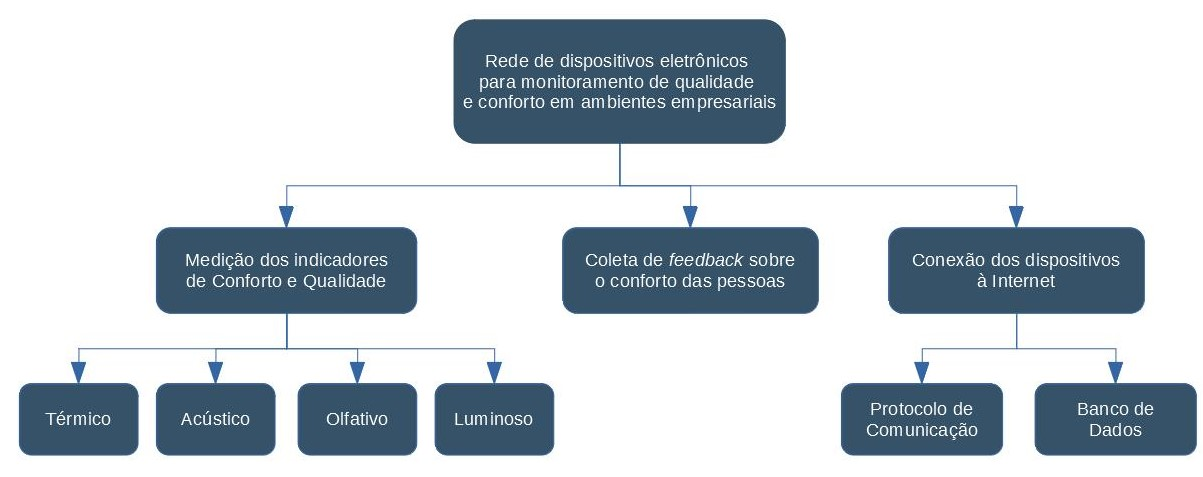
\includegraphics[scale=0.65]{objective_tree}
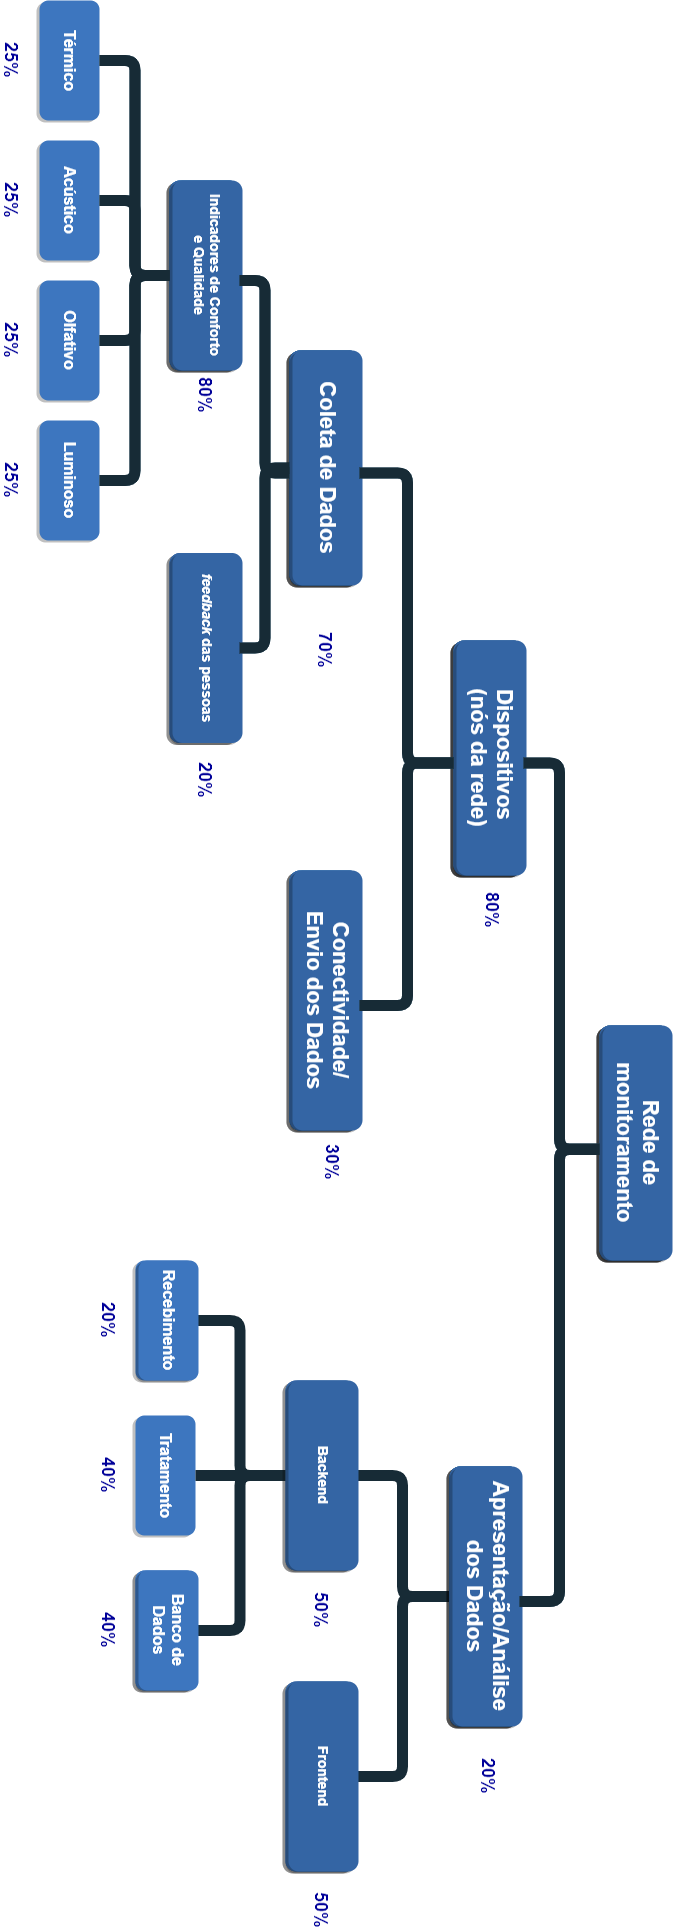
\includegraphics[width=\textwidth]{objective-tree-2}
\caption{Árvore de objetivos do projeto}
\label{fig:objective-tree}
\end{figure}


\end{document}